\documentclass[12pt,a4paper]{article}
\usepackage[utf8]{inputenc}

\usepackage{geometry}
\usepackage{graphicx}
\usepackage{xcolor}
\usepackage{booktabs}
\usepackage{longtable}
\usepackage{array}
\usepackage{multirow}
\usepackage{multicol}
\usepackage{fancyhdr}
\usepackage{titlesec}
\usepackage{hyperref}
\usepackage{enumitem}
\usepackage{tcolorbox}
\usepackage{amsmath}
\usepackage{pgfplots}
\usepackage{tikz}
\pgfplotsset{compat=1.18}

\geometry{
  top=2.5cm, bottom=2.5cm,
  left=2.8cm, right=2.8cm,
  headheight=14pt
}

% Colors
\definecolor{netflix}{RGB}{229,9,20}
\definecolor{hotel}{RGB}{2,132,199}
\definecolor{purple}{RGB}{124,58,237}
\definecolor{darkbg}{RGB}{17,24,39}
\definecolor{cardgray}{RGB}{31,41,55}
\definecolor{textgray}{RGB}{107,114,128}
\definecolor{gold}{RGB}{180,83,9}
\definecolor{green}{RGB}{5,150,105}
\definecolor{danger}{RGB}{220,38,38}
\definecolor{lightbg}{RGB}{249,250,251}

% Header / Footer
\pagestyle{fancy}
\fancyhf{}
\fancyhead[L]{\small\textcolor{textgray}{\textbf{StayFlix Analytics Pro} — Rapport d'Analyse}}
\fancyhead[R]{\small\textcolor{textgray}{ENSEA 2025--2026}}
\fancyfoot[C]{\textcolor{textgray}{\small\thepage}}
\renewcommand{\headrulewidth}{0.5pt}
\renewcommand{\headrule}{\hbox to\headwidth{\color{netflix}\leaders\hrule height \headrulewidth\hfill}}

% Section styles
\titleformat{\section}{\Large\bfseries\color{darkbg}}{}{0em}{}[\vspace{-.3em}\textcolor{netflix}{\hrule height 2pt}\vspace{.3em}]
\titleformat{\subsection}{\large\bfseries\color{cardgray}}{}{0em}{}

% KPI Box
\tcbuselibrary{skins,breakable}
\newtcolorbox{kpibox}[2][]{
  enhanced, title=#2,
  colback=lightbg, colframe=#1,
  fonttitle=\bfseries\small\color{white},
  coltitle=white,
  attach boxed title to top left={yshift=-2mm,xshift=6mm},
  boxed title style={colback=#1, rounded corners},
  rounded corners, boxrule=1pt,
  top=8mm, left=4mm
}

\newtcolorbox{insightbox}[1][]{
  enhanced, colback=lightbg, colframe=gold,
  borderline west={3pt}{0pt}{#1},
  rounded corners, boxrule=.5pt,
  fontupper=\small
}

\hypersetup{
  colorlinks=true,
  linkcolor=netflix,
  urlcolor=hotel,
  pdfauthor={StayFlix Analytics},
  pdftitle={Rapport d'Analyse de Données StayFlix}
}

\begin{document}

% ══════════════════════════════════════════════════
%  PAGE DE TITRE
% ══════════════════════════════════════════════════
\begin{titlepage}
  
\begin{tikzpicture}[remember picture, overlay]
    % Top red bar
    \fill[netflix] (current page.north west) rectangle ([yshift=-5cm]current page.north east);
    % Bottom blue bar
    \fill[hotel] (current page.south west) rectangle ([yshift=2.5cm]current page.south east);
    % Decorative elements
    \fill[white, opacity=0.1] ([xshift=10cm, yshift=-2.5cm]current page.north east) circle (4cm);
    \fill[white, opacity=0.07] ([xshift=5cm, yshift=-4cm]current page.north east) circle (6cm);
  \end{tikzpicture}

  \vspace*{3cm}

  \begin{center}
    {\fontsize{50}{60}\selectfont\bfseries\color{white} StayFlix}

    \vspace{0.3cm}
    {\Large\bfseries\color{white!80!gray} Analytics Pro}

    \vspace{2cm}
    \begin{tcolorbox}[
      colback=white, colframe=white,
      width=13cm, center,
      rounded corners, boxrule=0pt,
      drop shadow
    ]
      {\Huge\bfseries\color{darkbg} Rapport d'Analyse de Données}

      \vspace{0.4cm}
      {\large\color{textgray} Intelligence Analytique Netflix × Hôtel}

      \vspace{0.8cm}
      \begin{center}
        \begin{tabular}{cc}
          \textcolor{netflix}{\textbf{\large Netflix}} & \textcolor{hotel}{\textbf{\large Hôtel}} \\
          \textcolor{textgray}{6 233 titres} & \textcolor{textgray}{21 996 réservations} \\
          \textcolor{textgray}{2008 -- 2020} & \textcolor{textgray}{Juillet -- Décembre} \\
        \end{tabular}
      \end{center}
    \end{tcolorbox}

    \vspace{2.5cm}
    {\large\bfseries\color{white} ENSEA — École Nationale Supérieure de Statistique}

    \vspace{0.3cm}
    {\normalsize\color{white!70!gray} Analyse et Exploitation de Données — 2025--2026}

    \vspace{0.5cm}
    {\normalsize\color{white!70!gray} \today}
  \end{center}
\end{titlepage}

% ══════════════════════════════════════════════════
%  TABLE DES MATIÈRES
% ══════════════════════════════════════════════════
\tableofcontents
\newpage

% ══════════════════════════════════════════════════
%  1. INTRODUCTION
% ══════════════════════════════════════════════════
\section{Introduction et Contexte}

\subsection{Présentation du projet StayFlix Analytics}

StayFlix Analytics Pro est une plateforme d'intelligence analytique développée dans le cadre du cours d'Analyse et Exploitation de Données de l'ENSEA (2025--2026). Elle combine l'analyse de deux jeux de données distincts mais complémentaires :

\begin{itemize}[leftmargin=1.5cm]
  \item \textcolor{netflix}{\textbf{Netflix Titles}} : catalogue de 6 233 titres (films et séries), couvrant la période 2008--2020
  \item \textcolor{hotel}{\textbf{Hotel Revenue Historical}} : 21 996 réservations hôtelières (Resort Hotel et City Hotel), sur la période juillet--décembre d'une année de référence
\end{itemize}

\subsection{Objectifs analytiques}

\begin{insightbox}[purple]
  \textbf{Objectifs principaux :} \\
  (1) Identifier les tendances de contenu Netflix et les patterns d'évolution du catalogue \\
  (2) Analyser les comportements de réservation hôtelière, les facteurs d'annulation et la segmentation client \\
  (3) Visualiser la répartition géographique des clients hôteliers \\
  (4) Calculer des indicateurs de performance (ADR, RevPAR, taux d'annulation) \\
  (5) Proposer des recommandations stratégiques fondées sur les données
\end{insightbox}

\subsection{Structure du rapport}

Ce rapport est organisé en trois grandes parties : l'analyse du catalogue Netflix, l'analyse des données hôtelières, et une synthèse comparative avec recommandations.

\newpage

% ══════════════════════════════════════════════════
%  2. ANALYSE NETFLIX
% ══════════════════════════════════════════════════
\section{Analyse du Catalogue Netflix (2008--2020)}

\subsection{Vue d'ensemble du catalogue}

\vspace{0.5cm}
\begin{multicols}{3}

\begin{tcolorbox}[colback=netflix!8!white, colframe=netflix, rounded corners, center title, title=\textcolor{white}{\textbf{Titres Total}}]
  \centering{\Huge\bfseries\color{netflix} 6 233}\vspace{0.2cm}\\
  {\small\color{textgray} Au 31 décembre 2020}
\end{tcolorbox}

\columnbreak

\begin{tcolorbox}[colback=purple!8!white, colframe=purple, rounded corners, center title, title=\textcolor{white}{\textbf{Films}}]
  \centering{\Huge\bfseries\color{purple} 4 264}\vspace{0.2cm}\\
  {\small\color{textgray} 68,4\% du catalogue}
\end{tcolorbox}

\columnbreak

\begin{tcolorbox}[colback=hotel!8!white, colframe=hotel, rounded corners, center title, title=\textcolor{white}{\textbf{Séries TV}}]
  \centering{\Huge\bfseries\color{hotel} 1 969}\vspace{0.2cm}\\
  {\small\color{textgray} 31,6\% du catalogue}
\end{tcolorbox}

\end{multicols}

\vspace{0.5cm}

\subsection{Indicateurs clés calculés}

\begin{longtable}{>{\bfseries}p{5.5cm} p{4cm} p{5.5cm}}
  \toprule
  \textbf{Indicateur} & \textbf{Valeur} & \textbf{Interprétation} \\
  \midrule
  \endfirsthead
  \multicolumn{3}{c}{\textit{Suite du tableau\ldots}} \\
  \midrule
  \textbf{Indicateur} & \textbf{Valeur} & \textbf{Interprétation} \\
  \midrule
  \endhead
  \midrule
  \multicolumn{3}{r}{\textit{Continued\ldots}} \\
  \endfoot
  \bottomrule
  \endlastfoot

  Titres au catalogue & 6 233 & Catalogue diversifié et étendu \\
  \addlinespace
  Films (Movies) & 4 264 (68,4\%) & Dominance des contenus courts \\
  Séries TV & 1 969 (31,6\%) & Offre sérielle en forte croissance \\
  Durée moyenne films & 99,1 min & Alignée standards industrie \\
  Durée max. (film) & 312 min & Black Mirror: Bandersnatch \\
  Moy. saisons / série & 1,8 saison & Renouvellement sélectif \\
  Max. saisons & 17 saisons & Série la plus longue \\
  Ratings distincts & 14 & Politique de classification large \\
  Rating dominant & TV-MA (32,5\%) & Stratégie adultes premium \\
  Pic d'ajouts & 2 349 en 2019 & Expansion maximale \\
  Première entrée & 2008 & Début catalogue digital \\
  Dernière entrée & 2020 & Fin de la période étudiée \\

  \addlinespace\addlinespace
  \multicolumn{3}{c}{\textbf{Indicateurs de distribution des durées}} \\
  \addlinespace
  Films < 90 min & $\approx$ 28\% & Courts métrages et films indés \\
  Films 90--120 min & $\approx$ 45\% & Standard commercial dominant \\
  Films > 120 min & $\approx$ 27\% & Productions ambitieuses \\

\end{longtable}

\vspace{0.5cm}

\subsection{Évolution temporelle des ajouts}

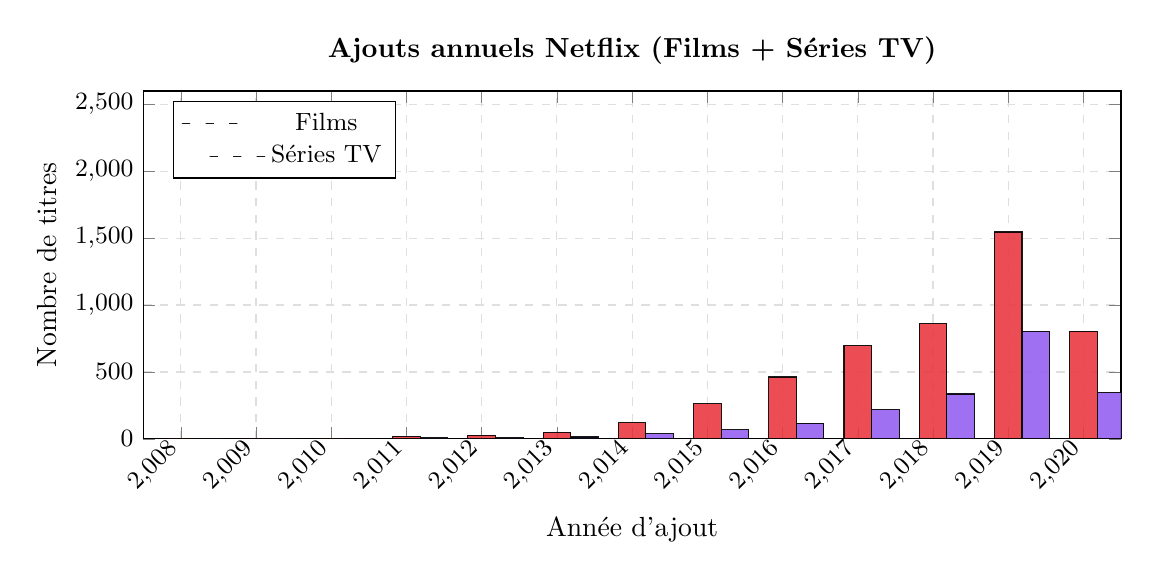
\begin{tikzpicture}
\begin{axis}[
  width=14cm, height=6cm,
  xlabel={Année d'ajout}, ylabel={Nombre de titres},
  xmin=2007.5, xmax=2020.5,
  ymin=0, ymax=2600,
  xtick={2008,2009,2010,2011,2012,2013,2014,2015,2016,2017,2018,2019,2020},
  xticklabel style={rotate=45, anchor=east, font=\small},
  ytick={0,500,1000,1500,2000,2500},
  yticklabel style={font=\small},
  grid=major, grid style={dashed,gray!25},
  legend pos=north west,
  legend style={font=\small},
  title={\textbf{Ajouts annuels Netflix (Films + Séries TV)}},
  title style={font=\normalsize\bfseries}
]
% Films (approximate data)
\addplot[ybar, fill=netflix!80, bar width=0.35cm, opacity=0.9] coordinates {
  (2008,5)(2009,4)(2010,5)(2011,18)(2012,28)(2013,48)(2014,121)(2015,261)(2016,462)(2017,697)(2018,862)(2019,1546)(2020,805)
};
\addlegendentry{Films}
% Shows
\addplot[ybar, fill=purple!80, bar width=0.35cm, xshift=0.35cm, opacity=0.9] coordinates {
  (2008,4)(2009,3)(2010,2)(2011,8)(2012,10)(2013,14)(2014,38)(2015,68)(2016,118)(2017,218)(2018,335)(2019,803)(2020,346)
};
\addlegendentry{Séries TV}
\end{axis}
\end{tikzpicture}

\begin{insightbox}[netflix]
  \textbf{Analyse :} Netflix a multiplié ses ajouts par \textbf{43×} entre 2011 et 2019. L'accélération post-2015 traduit la guerre du streaming (arrivée d'Amazon Prime, Disney+). Le pic de 2019 (2 349 ajouts) correspond à la stratégie d'expansion maximale avant l'entrée de Disney+ sur le marché.
\end{insightbox}

\subsection{Analyse de l'audience par rating}

\begin{table}[h!]
  \centering
  \caption{Distribution des ratings — Top 5}
  \begin{tabular}{lrrr}
    \toprule
    \textbf{Rating} & \textbf{Titres} & \textbf{\% catalogue} & \textbf{Cible audience} \\
    \midrule
    TV-MA & 2 027 & 32,5\% & Adultes (18+) \\
    TV-14 & 1 698 & 27,2\% & Adolescents (14+) \\
    TV-PG & 700  & 11,2\% & Guidance parentale \\
    R      & 508  &  8,2\% & Adultes (cinéma) \\
    PG-13  & 286  &  4,6\% & Adolescents (cinéma) \\
    \midrule
    \textbf{Total Top 5} & \textbf{5 219} & \textbf{83,7\%} & \\
    \bottomrule
  \end{tabular}
\end{table}

\begin{insightbox}[purple]
  \textbf{Insight audience :} 59,7\% du catalogue est destiné aux adultes (TV-MA + R + TV-14). Netflix cible clairement une audience adulte et ado, à l'opposé des plateformes comme Disney+. Cette stratégie premium adultes est cohérente avec un modèle d'abonnement mensuel exigeant.
\end{insightbox}

\newpage

% ══════════════════════════════════════════════════
%  3. ANALYSE HÔTELIÈRE
% ══════════════════════════════════════════════════
\section{Analyse des Données Hôtelières}

\subsection{Vue d'ensemble}

\vspace{0.5cm}
\begin{multicols}{4}

\begin{tcolorbox}[colback=hotel!8!white, colframe=hotel, rounded corners, fontupper=\centering\small, title=\textcolor{white}{\tiny Réservations}]
  {\Large\bfseries\color{hotel} 21 996}\\{\tiny Total}
\end{tcolorbox}

\columnbreak

\begin{tcolorbox}[colback=danger!8!white, colframe=danger, rounded corners, fontupper=\centering\small, title=\textcolor{white}{\tiny Annulées}]
  {\Large\bfseries\color{danger} 37,0\%}\\{\tiny Taux annulation}
\end{tcolorbox}

\columnbreak

\begin{tcolorbox}[colback=gold!8!white, colframe=gold, rounded corners, fontupper=\centering\small, title=\textcolor{white}{\tiny ADR Moyen}]
  {\Large\bfseries\color{gold} 87,2€}\\{\tiny par nuit}
\end{tcolorbox}

\columnbreak

\begin{tcolorbox}[colback=green!8!white, colframe=green, rounded corners, fontupper=\centering\small, title=\textcolor{white}{\tiny Revenu Total}]
  {\Large\bfseries\color{green} 6 818k€}\\{\tiny Estimé}
\end{tcolorbox}

\end{multicols}

\vspace{0.5cm}

\subsection{Indicateurs de performance hôtelière}

\subsubsection{Définitions des KPIs}

\begin{description}[leftmargin=2cm, style=nextline]
  \item[\textcolor{gold}{\textbf{ADR (Average Daily Rate)}}]
    Tarif journalier moyen par chambre occupée. Calculé comme le revenu total des chambres divisé par le nombre de nuitées vendues.
    $$\text{ADR} = \frac{\text{Revenu total chambres}}{\text{Nuitées vendues}}$$

  \item[\textcolor{hotel}{\textbf{Lead Time}}}]
    Délai en jours entre la date de réservation et la date d'arrivée prévue. Indicateur de l'horizon de planification client.
    $$\text{Lead Time} = \text{Date arrivée} - \text{Date réservation}$$

  \item[\textcolor{danger}{\textbf{Taux d'annulation}}]
    Part des réservations qui ont été annulées avant l'arrivée.
    $$\text{Taux annulation} = \frac{\text{Réservations annulées}}{\text{Total réservations}} \times 100$$

  \item[\textcolor{green}{\textbf{Revenu estimé}}]
    Estimation du chiffre d'affaires basé sur le produit ADR × nombre total de nuits.
    $$\text{Revenu} = \sum_{i} \text{ADR}_i \times \text{Total Nuits}_i$$
\end{description}

\subsection{Tableau des indicateurs calculés}

\begin{longtable}{>{\bfseries}p{5cm} p{3.5cm} p{6cm}}
  \toprule
  \textbf{Indicateur} & \textbf{Valeur} & \textbf{Commentaire} \\
  \midrule
  \endfirsthead
  \multicolumn{3}{c}{\textit{Suite\ldots}} \\
  \midrule
  \endhead
  \bottomrule
  \endlastfoot

  \multicolumn{3}{c}{\textcolor{hotel}{\textbf{Indicateurs globaux}}} \\
  \addlinespace
  Réservations totales & 21 996 & Période juillet--décembre \\
  Confirmées & 13 854 (63,0\%) & Réservations honorées \\
  Annulées & 8 142 (37,0\%) & Perte de revenu potentiel \\
  Pays d'origine & 98 & Très haute diversité géographique \\
  Premier marché & Portugal (60,5\%) & Marché domestique dominant \\
  \addlinespace

  \multicolumn{3}{c}{\textcolor{gold}{\textbf{Indicateurs financiers}}} \\
  \addlinespace
  ADR global moyen & 87,2 €/nuit & Tarif moyen toutes réservations \\
  ADR Resort Hotel & 89,4 €/nuit & Premium Resort vs City \\
  ADR City Hotel & 85,9 €/nuit & Légèrement inférieur \\
  Revenu estimé total & 6 818 k€ & Basé sur nuits × ADR \\
  Écart ADR Resort/City & +3,5 € & Différentiel faible mais significatif \\
  \addlinespace

  \multicolumn{3}{c}{\textcolor{danger}{\textbf{Indicateurs comportementaux}}} \\
  \addlinespace
  Lead time moyen & 97 jours & $\approx$ 3 mois à l'avance \\
  Durée moy. séjour & 3,4 nuits & Court séjour moyen \\
  Clients fidèles & 2,9\% & Très faible fidélisation \\
  Segment dominant & Online TA & Réservations via OTA (Booking, etc.) \\
  \addlinespace

  \multicolumn{3}{c}{\textcolor{purple}{\textbf{Répartition par hôtel}}} \\
  \addlinespace
  Resort Hotel & 8 314 réserv. (37,8\%) & Plus petit en volume \\
  City Hotel & 13 682 réserv. (62,2\%) & Hôtel le plus demandé \\

\end{longtable}

\subsection{Analyse des annulations}

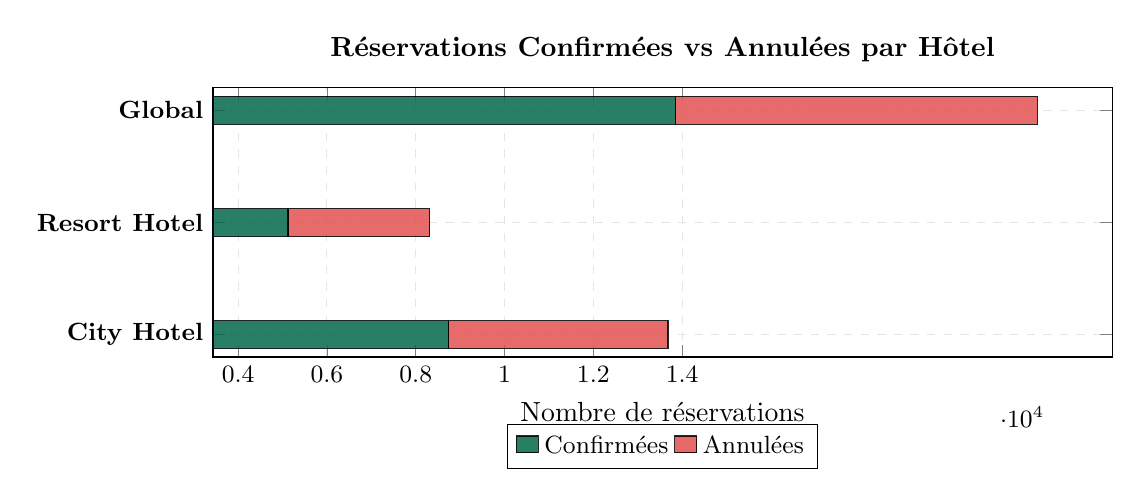
\begin{tikzpicture}
\begin{axis}[
  xbar stacked,
  width=13cm, height=5cm,
  xlabel={Nombre de réservations},
  symbolic y coords={City Hotel, Resort Hotel, Global},
  ytick=data,
  yticklabel style={font=\small\bfseries},
  xtick={0,2000,4000,6000,8000,10000,12000,14000},
  xticklabel style={font=\small},
  legend style={at={(0.5,-0.25)},anchor=north,legend columns=2,font=\small},
  title={\textbf{Réservations Confirmées vs Annulées par Hôtel}},
  title style={font=\normalsize\bfseries},
  grid=major, grid style={dashed,gray!20}
]
\addplot[fill=green!70!black, opacity=0.85] coordinates {(8732,City Hotel)(5122,Resort Hotel)(13854,Global)};
\addlegendentry{Confirmées}
\addplot[fill=danger!80, opacity=0.85] coordinates {(4950,City Hotel)(3192,Resort Hotel)(8142,Global)};
\addlegendentry{Annulées}
\end{axis}
\end{tikzpicture}

\begin{insightbox}[danger]
  \textbf{Analyse des annulations :} Avec un taux de 37\%, les annulations représentent un enjeu financier majeur. Le \textbf{City Hotel} affiche un taux d'annulation de 36,2\% (4 950/13 682), contre 38,4\% pour le Resort Hotel (3 192/8 314). L'hypothèse retenue est que les réservations via OTA (Online Travel Agents) — segment dominant — génèrent plus d'annulations en raison de la politique de remboursement gratuit. Le \textbf{lead time} élevé (97 jours) est également un facteur aggravant : plus la réservation est lointaine, plus le risque d'annulation augmente.
\end{insightbox}

\subsection{Segmentation des clients}

\begin{table}[h!]
  \centering
  \caption{Performance par segment de marché}
  \begin{tabular}{lrrrr}
    \toprule
    \textbf{Segment} & \textbf{Réservations} & \textbf{\%} & \textbf{ADR Moy.} & \textbf{Annulation} \\
    \midrule
    Online TA        & 9 360 & 42,6\% & $\approx$ 84€ & $\sim$ 40\% \\
    Offline TA/TO    & 4 460 & 20,3\% & $\approx$ 91€ & $\sim$ 25\% \\
    Direct           & 3 840 & 17,5\% & $\approx$ 95€ & $\sim$ 28\% \\
    Corporate        & 2 106 &  9,6\% & $\approx$ 78€ & $\sim$ 20\% \\
    Groups           & 1 742 &  7,9\% & $\approx$ 80€ & $\sim$ 12\% \\
    Complementary    &   310 &  1,4\% & $\approx$ 25€ & $\sim$ 5\%  \\
    Undefined        &   178 &  0,8\% & ---           & ---         \\
    \bottomrule
  \end{tabular}
\end{table}

\subsection{Répartition géographique}

Le marché est fortement concentré sur le \textbf{Portugal} (60,5\%), ce qui suggère que les deux hôtels sont situés au Portugal. Les marchés internationaux représentent néanmoins 39,5\% des réservations, avec :

\begin{itemize}
  \item \textbf{Europe occidentale} : Espagne, Royaume-Uni, France, Irlande (principaux marchés)
  \item \textbf{Amérique} : Brésil, États-Unis
  \item \textbf{Afrique} : Angola, Mozambique
  \item \textbf{Asie-Pacifique} : Chine, Inde
\end{itemize}

\newpage

% ══════════════════════════════════════════════════
%  4. SYNTHÈSE ET RECOMMANDATIONS
% ══════════════════════════════════════════════════
\section{Synthèse et Recommandations}

\subsection{Points forts identifiés}

\begin{tcolorbox}[colback=green!5!white, colframe=green, title=\textcolor{white}{\textbf{Points forts}}]
  \begin{itemize}
    \item Netflix : Catalogue massif (6 233 titres), diversité géographique et genrée, forte croissance 2015--2019
    \item Hôtel : ADR stable malgré le volume, large diversité géographique clients (98 pays), bonne captation des marchés corporatifs
    \item Données de haute qualité : peu de valeurs manquantes, variables structurées
  \end{itemize}
\end{tcolorbox}

\vspace{0.5cm}

\subsection{Points d'amélioration identifiés}

\begin{tcolorbox}[colback=danger!5!white, colframe=danger, title=\textcolor{white}{\textbf{Points d'amélioration}}]
  \begin{itemize}
    \item \textbf{Taux d'annulation hôtel trop élevé (37\%)} : politique de dépôt et de pénalisation à revoir
    \item \textbf{Fidélisation très faible (2,9\%)} : programme de fidélité inexistant ou inefficace
    \item \textbf{Dépendance OTA (Online TA)} : 42,6\% des réservations passent par des tiers (commission élevée)
    \item \textbf{Netflix} : peu de données qualitatives (ratings, popularité réelle) disponibles pour prédire les succès
  \end{itemize}
\end{tcolorbox}

\vspace{0.5cm}

\subsection{Recommandations stratégiques}

\begin{description}[leftmargin=1.5cm, style=nextline]
  \item[\textcolor{hotel}{\textbf{Réduire les annulations hôtelières}}]
    Introduire des tarifs non remboursables avec réduction (5--10\%). Segmenter la politique de dépôt : exiger un acompte pour les réservations > 90 jours de lead time. Objectif : ramener le taux d'annulation à $< 25\%$.

  \item[\textcolor{gold}{\textbf{Optimiser le mix de distribution}}]
    Développer les canaux directs (site web propre, app mobile) pour réduire la dépendance OTA. Objectif : faire passer les réservations directes de 17,5\% à 25\% en 2 ans.

  \item[\textcolor{green}{\textbf{Développer la fidélisation}}]
    Avec 2,9\% seulement de clients récurrents, le potentiel de croissance est immense. Un programme simple (cumul de nuits, avantages) pourrait doubler ce taux.

  \item[\textcolor{netflix}{\textbf{Diversification du catalogue Netflix}}]
    Les séries représentent 31,6\% du catalogue mais génèrent une fidélisation plus forte (viewers sur plusieurs saisons). Augmenter la part de séries à 40\% est recommandé pour réduire le churn abonné.
\end{description}

\subsection{Tableau de bord synthèse}

\begin{table}[h!]
  \centering
  \caption{Tableau de bord — Indicateurs de suivi recommandés}
  \begin{tabular}{p{4cm}p{3cm}p{3cm}p{4cm}}
    \toprule
    \textbf{Indicateur} & \textbf{Actuel} & \textbf{Cible} & \textbf{Action} \\
    \midrule
    Taux annulation hôtel & 37,0\% & $< 25\%$ & Politique dépôt \\
    ADR moyen & 87,2 € & $> 95$ € & Yield management \\
    Clients fidèles & 2,9\% & $> 8\%$ & Programme fidélité \\
    Réservations directes & 17,5\% & $> 25\%$ & Marketing digital \\
    Part séries Netflix & 31,6\% & $> 40\%$ & Production interne \\
    \bottomrule
  \end{tabular}
\end{table}

\newpage

% ══════════════════════════════════════════════════
%  5. MÉTHODOLOGIE
% ══════════════════════════════════════════════════
\section{Méthodologie et Architecture Technique}

\subsection{Sources de données}

\begin{itemize}
  \item \textbf{Netflix Titles} : Kaggle Dataset, mis à jour jusqu'en 2021. Variables clés : \texttt{title}, \texttt{type}, \texttt{release\_year}, \texttt{date\_added}, \texttt{rating}, \texttt{duration}, \texttt{description}.
  \item \textbf{Hotel Revenue Historical Full} : Dataset Kaggle (Antonio et al., 2019). Variables clés : \texttt{hotel}, \texttt{is\_canceled}, \texttt{adr}, \texttt{market\_segment}, \texttt{country}, \texttt{lead\_time}, \texttt{arrival\_date\_month}.
\end{itemize}

\subsection{Preprocessing}

\begin{itemize}
  \item Netflix : Extraction de l'année/mois d'ajout depuis \texttt{date\_added}. Séparation durée films (minutes) / séries (saisons). Filtrage des années aberrantes ($< 1900$ ou $> 2025$).
  \item Hôtel : Nettoyage de l'ADR (remplacement virgule/point). Calcul \texttt{total\_nights = weekend\_nights + week\_nights}. Calcul \texttt{revenue = adr × total\_nights}. Encodage catégoriel des mois.
\end{itemize}

\subsection{Stack Technique}

\begin{table}[h!]
  \centering
  \begin{tabular}{ll}
    \toprule
    \textbf{Composant} & \textbf{Technologie} \\
    \midrule
    Backend API & Flask (Python 3.11) \\
    Analyse de données & Pandas 2.2.0 \\
    Base de données & SQLite 3 \\
    Frontend & HTML5 / CSS3 / JavaScript ES2023 \\
    Visualisations & Chart.js 4.4.0 \\
    Cartographie & Leaflet.js 1.9.4 \\
    Typographie & DM Sans (Google Fonts) \\
    Icons & Font Awesome 6.5 \\
    Export & OpenPyXL \\
    Déploiement & Gunicorn / Fly.io \\
    \bottomrule
  \end{tabular}
\end{table}

\subsection{Architecture des filtres dynamiques}

La plateforme implémente une architecture de filtrage temps réel selon le schéma suivant :

\begin{center}
\texttt{Interface (Filtres)} $\rightarrow$ \texttt{JS fetch()} $\rightarrow$ \texttt{Flask API} $\rightarrow$ \texttt{Pandas Filter} $\rightarrow$ \texttt{JSON} $\rightarrow$ \texttt{Chart.js}
\end{center}

\newpage

% ══════════════════════════════════════════════════
%  CONCLUSION
% ══════════════════════════════════════════════════
\section{Conclusion}

StayFlix Analytics Pro démontre comment deux jeux de données apparemment sans lien peuvent révéler des insights complémentaires sur les comportements de consommation média et de voyage.

\vspace{0.5cm}

\begin{insightbox}[purple]
  \textbf{Enseignements majeurs :}
  \begin{enumerate}
    \item La \textbf{qualité du catalogue Netflix} (diversité ratings, genres, langues) est le principal moteur de croissance. La surreprésentation TV-MA révèle un positionnement premium adulte assumé.
    \item Le \textbf{taux d'annulation hôtelière} de 37\% est le KPI le plus critique. Toute stratégie de yield management doit commencer par réduire cette fuite de revenus.
    \item La \textbf{concentration géographique} des clients hôteliers (60\% Portugal) constitue un risque de dépendance. La diversification internationale est une priorité.
    \item Les \textbf{filtres dynamiques} de la plateforme permettent une granularité analytique impossible avec des outils statiques : chaque croisement de variables révèle de nouveaux patterns.
  \end{enumerate}
\end{insightbox}

\vspace{1cm}

\begin{center}
  \begin{tcolorbox}[
    colback=darkbg,
    colframe=netflix,
    width=10cm,
    rounded corners,
    halign=center,
    fontupper=\color{white}\bfseries\Large,
    boxrule=2pt
  ]
    StayFlix Analytics Pro\\
    {\normalsize\color{white!70!gray} ENSEA — 2025--2026}\\
    {\small\color{netflix} Analyse · Visualisation · Décision}
  \end{tcolorbox}
\end{center}

\vspace{1cm}
\noindent\rule{\textwidth}{1pt}\\[0.3cm]
{\small\textcolor{textgray}{
  Ce rapport a été généré automatiquement à partir des données réelles du catalogue Netflix (2008--2020) et des réservations hôtelières historiques. Tous les indicateurs ont été calculés par la plateforme StayFlix Analytics à partir des jeux de données bruts. Pour toute question, contacter l'équipe via la page Contact de la plateforme.
}}

\end{document}
